\documentclass[12pt,ngerman]{scrartcl}

\usepackage[utf8]{inputenc}
\usepackage[T1]{fontenc}
\usepackage{booktabs}
\usepackage{babel}
\usepackage{graphicx}
\usepackage{csquotes}
\usepackage{paralist}
\usepackage{xcolor}

\usepackage[sfdefault]{plex-sans}

\usepackage{tikz}
\usetikzlibrary{arrows}
\usepackage{pgfplots}
\pgfplotsset{compat=1.12}

\begin{document}


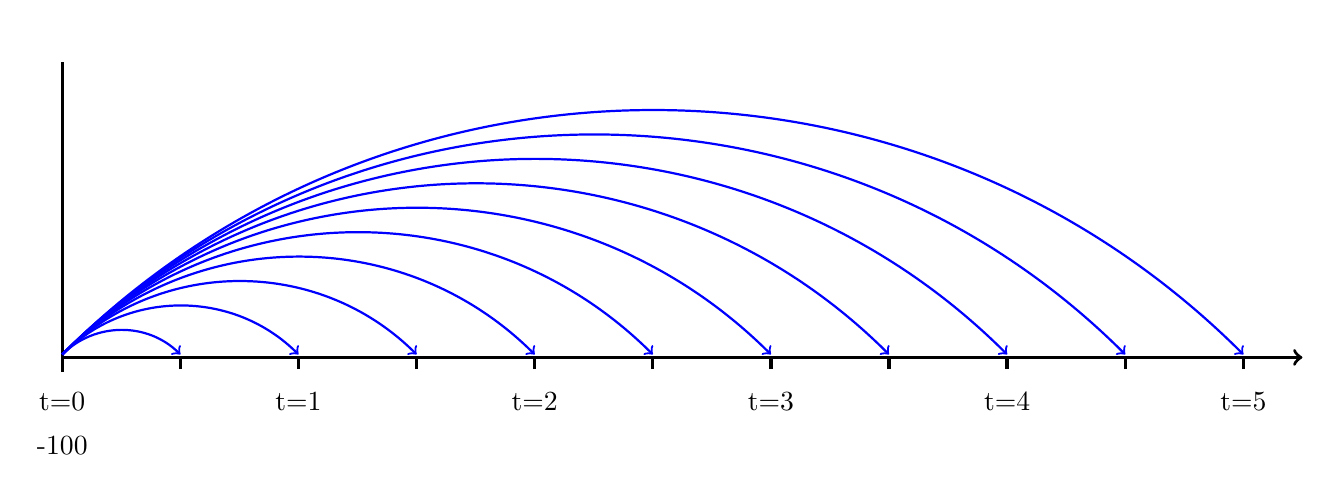
\begin{tikzpicture}[scale=0.75]
%\draw[step=1.0,red,thin] (-1,-1) grid (16,5);
\draw[very thick] (0,0.75) -- (0,6);
\draw[very thick,->] (0,1) -- (21,1);

\draw[very thick] (2,0.8) -- (2,1.0);
\draw[very thick] (4,0.8) -- (4,1.0);
\draw[very thick] (6,0.8) -- (6,1.0);
\draw[very thick] (8,0.8) -- (8,1.0);
\draw[very thick] (10,0.8) -- (10,1.0);
\draw[very thick] (12,0.8) -- (12,1.0);
\draw[very thick] (14,0.8) -- (14,1.0);
\draw[very thick] (16,0.8) -- (16,1.0);
\draw[very thick] (18,0.8) -- (18,1.0);
\draw[very thick] (20,0.8) -- (20,1.0);

\draw (0,0.25) node {t=0};
\draw (4,0.25) node {t=1};
\draw (8,0.25) node {t=2};
\draw (12,0.25) node {t=3};
\draw (16,0.25) node {t=4};
\draw (20,0.25) node {t=5};

\draw (0,-0.5) node {-100};

\draw[blue,thick,->] (0,1.05) to[bend left=-45,bend right = -45] (2,1.05);
\draw[blue,thick,->] (0,1.05) to[bend left=-45,bend right = -45] (4,1.05);
\draw[blue,thick,->] (0,1.05) to[bend left=-45,bend right = -45] (6,1.05);
\draw[blue,thick,->] (0,1.05) to[bend left=-45,bend right = -45] (8,1.05);
\draw[blue,thick,->] (0,1.05) to[bend left=-45,bend right = -45] (10,1.05);
\draw[blue,thick,->] (0,1.05) to[bend left=-45,bend right = -45] (12,1.05);
\draw[blue,thick,->] (0,1.05) to[bend left=-45,bend right = -45] (14,1.05);
\draw[blue,thick,->] (0,1.05) to[bend left=-45,bend right = -45] (16,1.05);
\draw[blue,thick,->] (0,1.05) to[bend left=-45,bend right = -45] (18,1.05);
\draw[blue,thick,->] (0,1.05) to[bend left=-45,bend right = -45] (20,1.05);


\end{tikzpicture}

\vspace*{2cm}

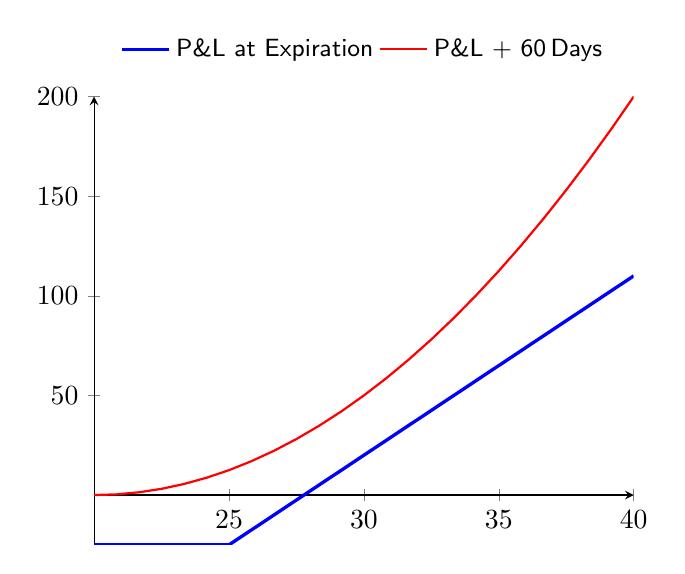
\begin{tikzpicture}[
font=\sffamily,
  declare function={
    mypl(\x)= -25 + (\x>25) * (9*(\x-25));
  }
]
\begin{axis}[
  domain=20:40,
  axis lines=middle,
  legend style={
    draw=none,
    legend columns=-1,
    at={(0.5,1)},
    anchor=south,
    outer sep=1em,
    node font=\small,
  },
]
  \addplot[blue,very thick] {mypl(x)};
  \addlegendentry{P\&L at Expiration}
  \addplot[red,thick] {0.5*(x-20)^2};
  \addlegendentry{P\&L + 60\,Days};
\end{axis}
\end{tikzpicture}



\end{document}